\section{Smartphone Application}

\begin{figure}
    \center
    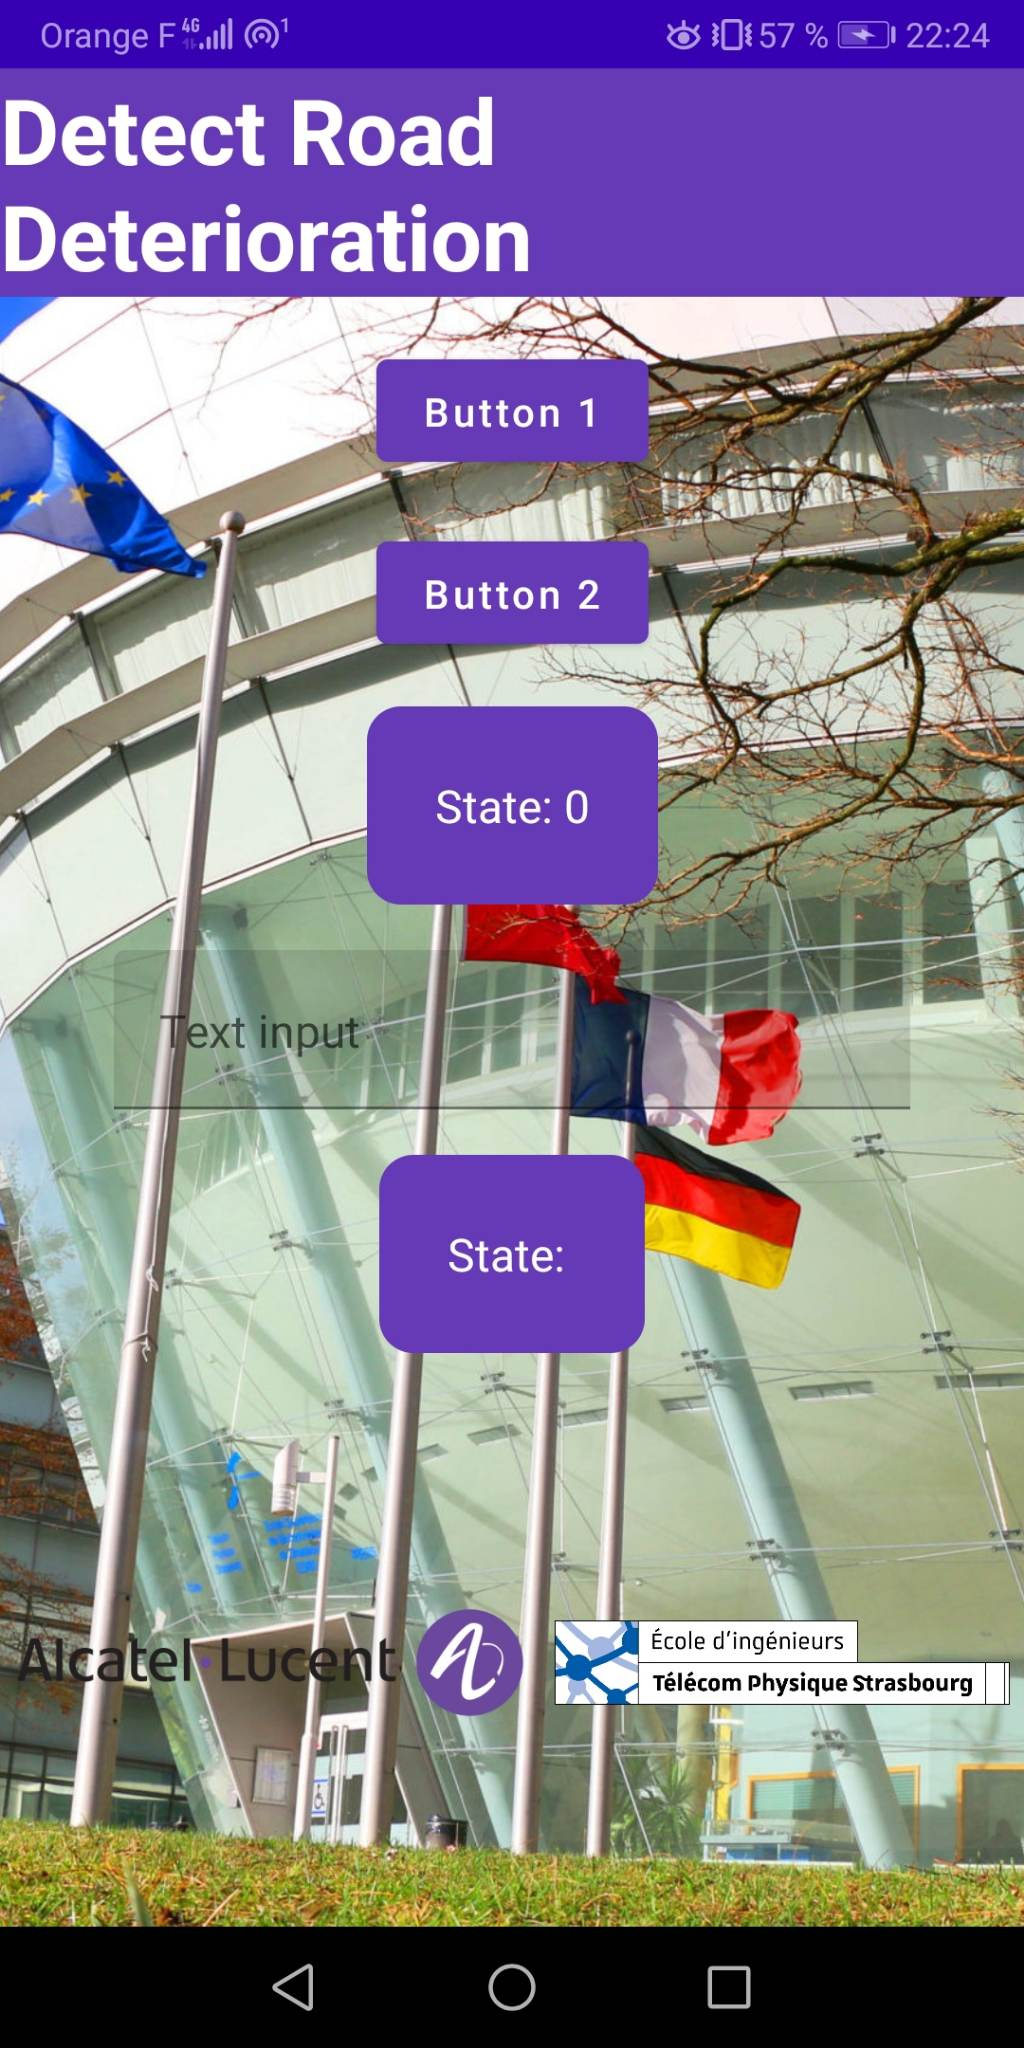
\includegraphics[scale=.12]{img/test_app.jpg}
    \caption{First Android application made using Android Studio}
    \label{app}
\end{figure}

The developement of the application will have to start during the next sprint and continue throughout the rest of the project in parallel with the other tasks.This process will take a lot of time because none of us has any experience what so ever regarding developing smartphone application.\\
We made a few research on that subject and settled for developing an Android application using Android Studio as we do not have any Apple device and Android Studio combines all the tools required for developing a proper application. By following a couple of tutorials on the Android Developers website we managed to build a rather nice looking (but useless) application (Figure \ref{app}).